\documentclass[a4paper,10pt]{report}

\usepackage{bold-extra}

\usepackage[utf8x]{inputenc}

\usepackage[cm]{fullpage}

\usepackage{graphicx}
\usepackage{subfig}
\usepackage{amsmath}
%\usepackage{mathtools}

%opening
%\title{Contact Angles and Line Tension of different SAMs via the Droplet Method}
%\author{Laila Eixeres}

\everymath{\displaystyle}

\begin{document}

%\maketitle



\begin{figure}
%\centering
{\Large SAMs with 0\% OH-coverage.}
\newline
\subfloat{
  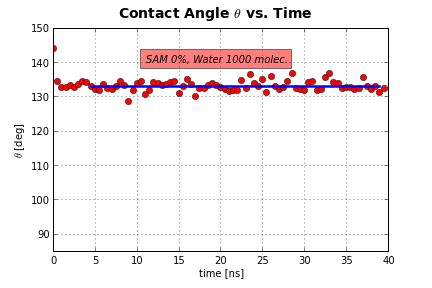
\includegraphics[width=95mm]{thetas0w1000}
}
\subfloat{
  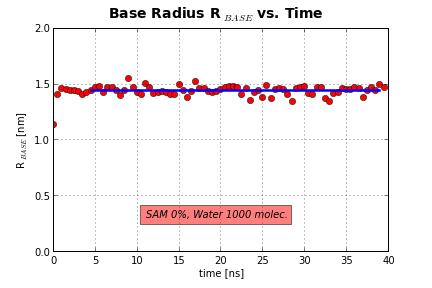
\includegraphics[width=95mm]{rads0w1000}
}
\newline
\subfloat{
  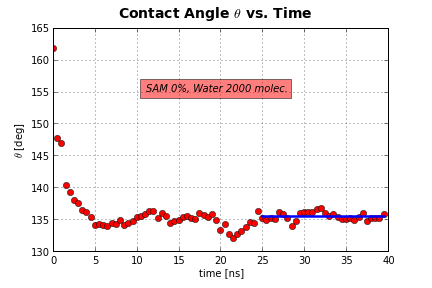
\includegraphics[width=95mm]{thetas0w2000}
}
\subfloat{
  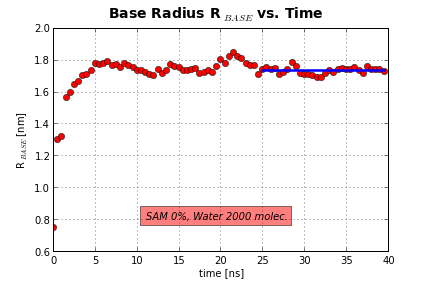
\includegraphics[width=95mm]{rads0w2000}
}
\newline
\subfloat{
  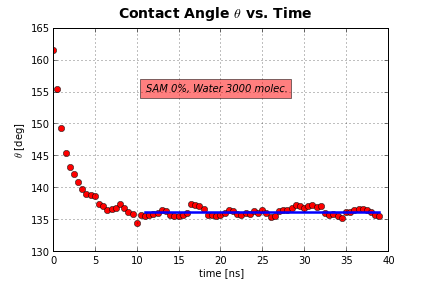
\includegraphics[width=95mm]{thetas0w3000}
}
\subfloat{
  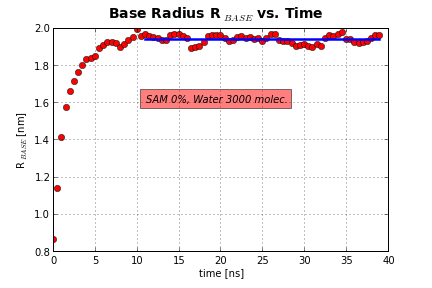
\includegraphics[width=95mm]{rads0w3000}
}
\newline
\subfloat{
  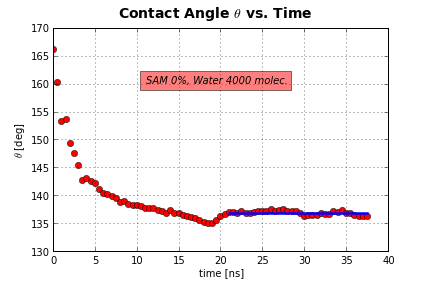
\includegraphics[width=95mm]{thetas0w4000}
}
\subfloat{
  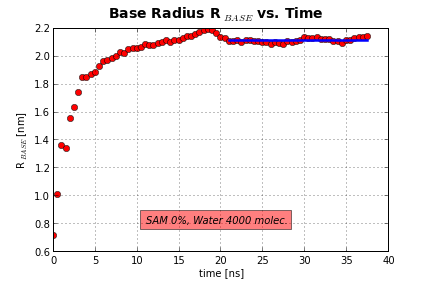
\includegraphics[width=95mm]{rads0w4000}
}
\end{figure}
\pagebreak
\begin{figure}
\subfloat{
  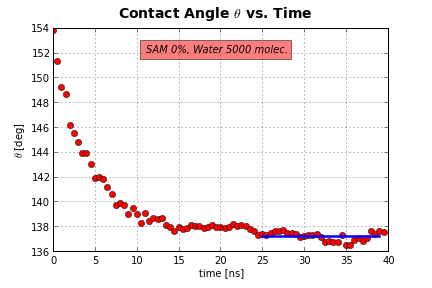
\includegraphics[width=95mm]{thetas0w5000}
}
\subfloat{
  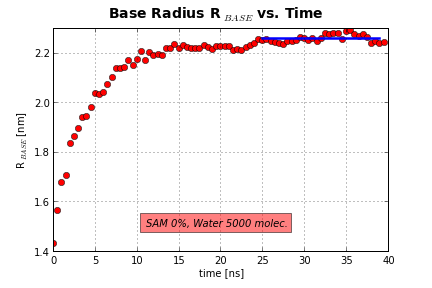
\includegraphics[width=95mm]{rads0w5000}
}
\newline
\subfloat{
  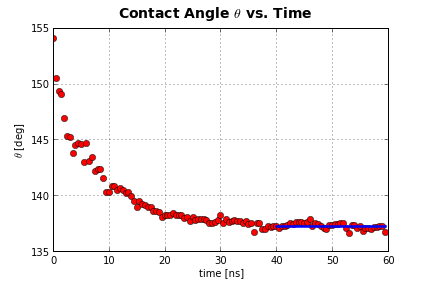
\includegraphics[width=95mm]{thetas0w6500}
}
\subfloat{
  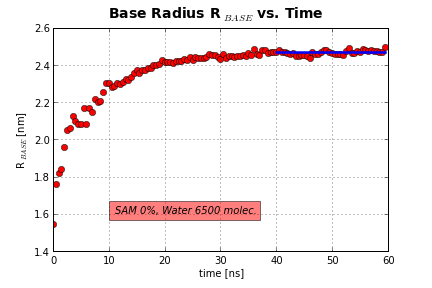
\includegraphics[width=95mm]{rads0w6500}
}
\newline
\subfloat{
  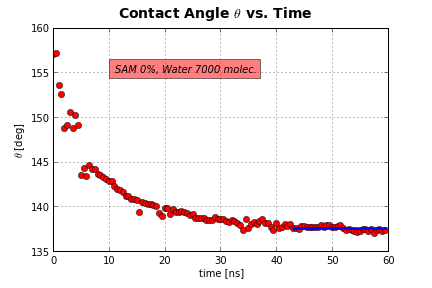
\includegraphics[width=95mm]{thetas0w7000}
}
\subfloat{
  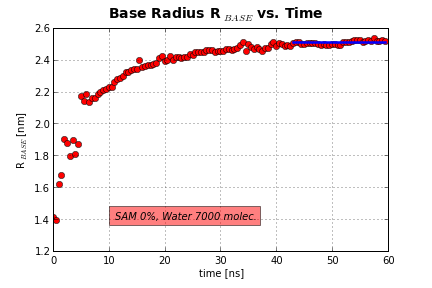
\includegraphics[width=95mm]{rads0w7000}
}
\newline
\subfloat{
  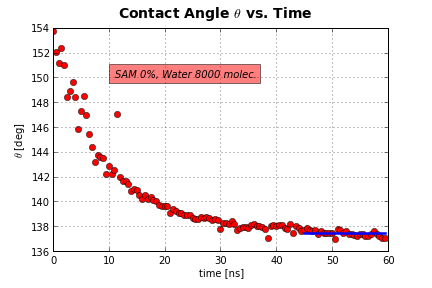
\includegraphics[width=95mm]{thetas0w8000}
}
\subfloat{
  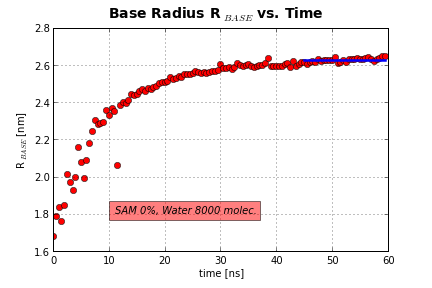
\includegraphics[width=95mm]{rads0w8000}
}
\end{figure}

\begin{figure}
\subfloat{
  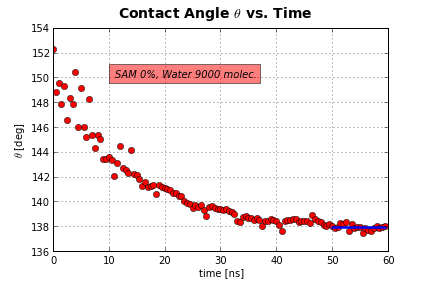
\includegraphics[width=95mm]{thetas0w9000}
}
\subfloat{
  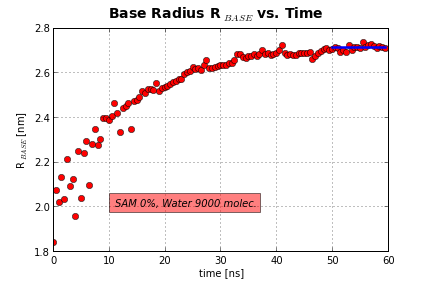
\includegraphics[width=95mm]{rads0w9000}
}
\newline
\subfloat{
  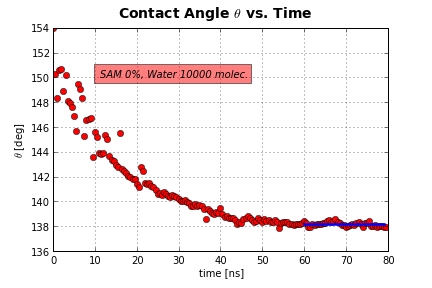
\includegraphics[width=95mm]{thetas0w10000}
}
\subfloat{
  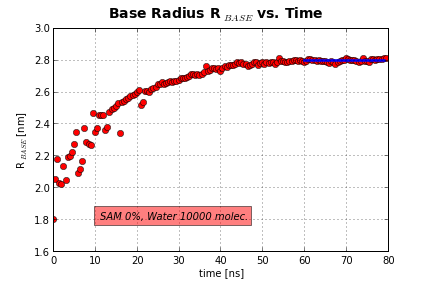
\includegraphics[width=95mm]{rads0w10000}
}
\newline
%\centering
{\Large SAMs with 5\% OH-coverage.}
\newline
\subfloat{
  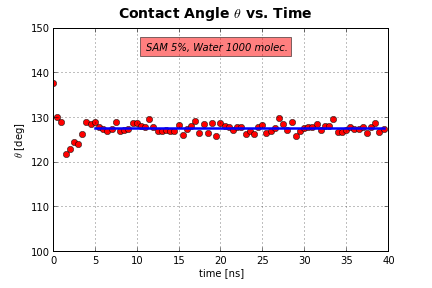
\includegraphics[width=95mm]{thetas5w1000}
}
\subfloat{
  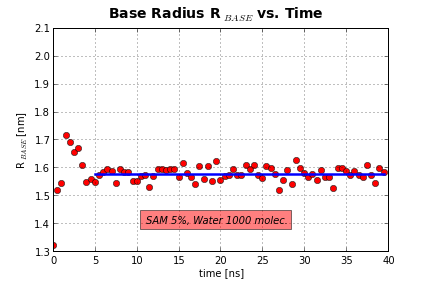
\includegraphics[width=95mm]{rads5w1000}
}
\newline
\subfloat{
  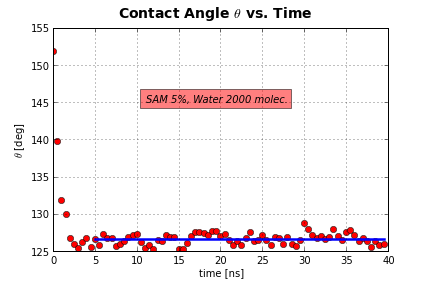
\includegraphics[width=95mm]{thetas5w2000}
}
\subfloat{
  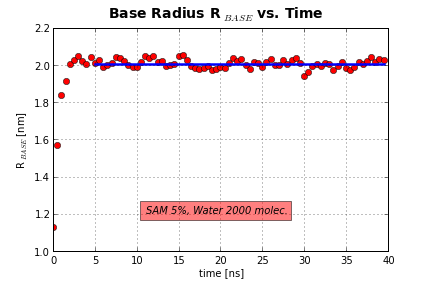
\includegraphics[width=95mm]{rads5w2000}
}
\end{figure}
\begin{figure}
\subfloat{
  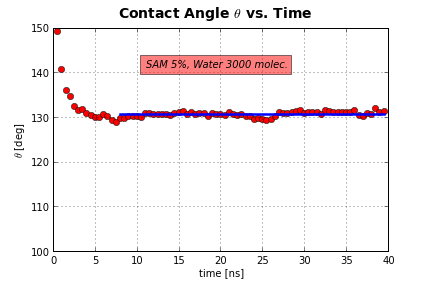
\includegraphics[width=95mm]{thetas5w3000}
}
\subfloat{
  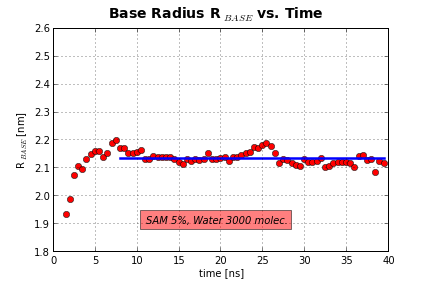
\includegraphics[width=95mm]{rads5w3000}
}
\newline
\subfloat{
  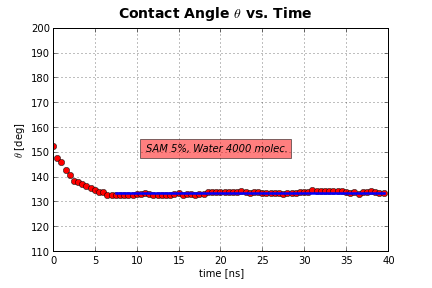
\includegraphics[width=95mm]{thetas5w4000}
}
\subfloat{
  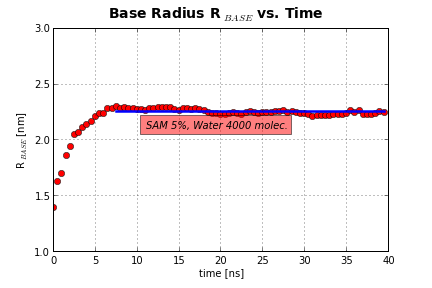
\includegraphics[width=95mm]{rads5w4000}
}
\newline
\subfloat{
  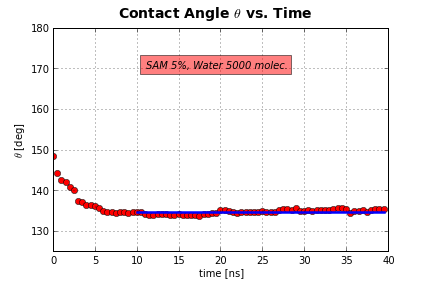
\includegraphics[width=95mm]{thetas5w5000}
}
\subfloat{
  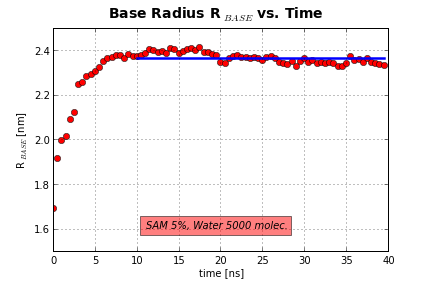
\includegraphics[width=95mm]{rads5w5000}
}
\newline
\subfloat{
  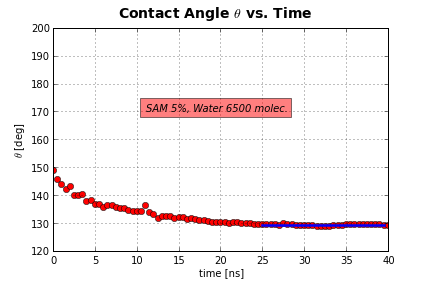
\includegraphics[width=95mm]{thetas5w6500}
}
\subfloat{
  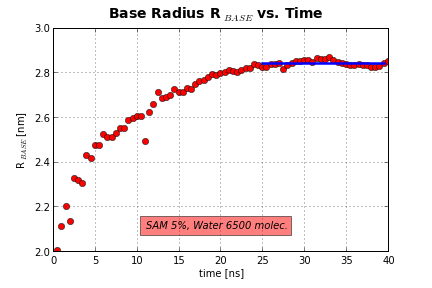
\includegraphics[width=95mm]{rads5w6500}
}
\end{figure}
\begin{figure}
\subfloat{
  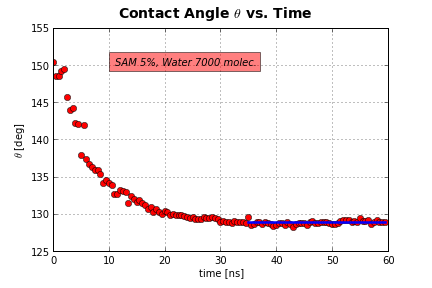
\includegraphics[width=95mm]{thetas5w7000}
}
\subfloat{
  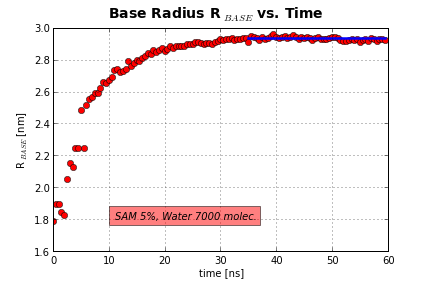
\includegraphics[width=95mm]{rads5w7000}
}
\newline
\subfloat{
  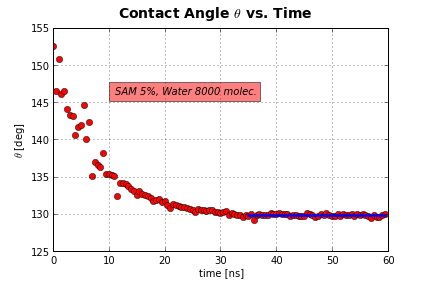
\includegraphics[width=95mm]{thetas5w8000}
}
\subfloat{
  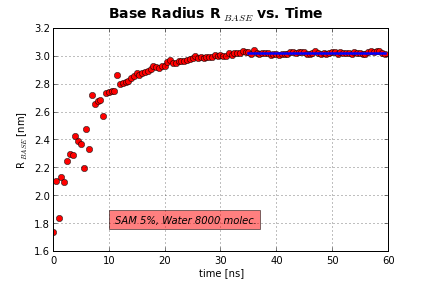
\includegraphics[width=95mm]{rads5w8000}
}
\newline
\subfloat{
  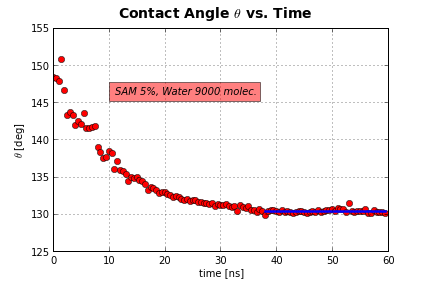
\includegraphics[width=95mm]{thetas5w9000}
}
\subfloat{
  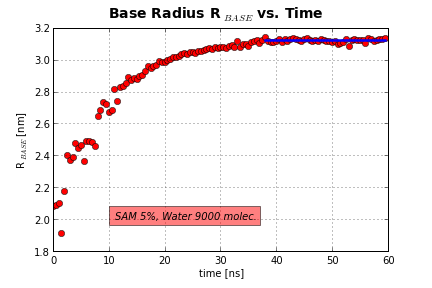
\includegraphics[width=95mm]{rads5w9000}
}
\newline
\subfloat{
  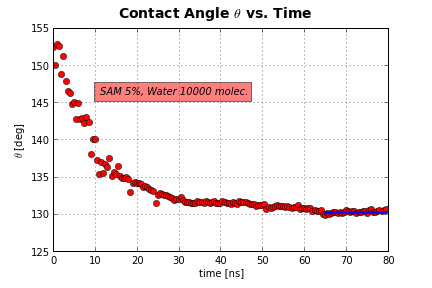
\includegraphics[width=95mm]{thetas5w10000}
}
\subfloat{
  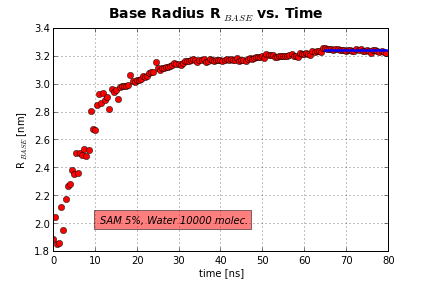
\includegraphics[width=95mm]{rads5w10000}
}
\end{figure}

\begin{figure}
%\centering
{\Large SAMs with 11\% OH-coverage.}
\newline
\subfloat{
  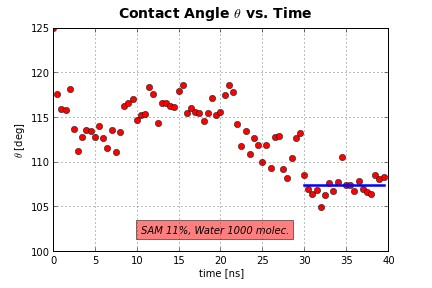
\includegraphics[width=95mm]{thetas11w1000}
}
\subfloat{
  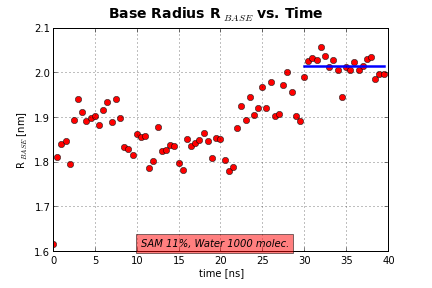
\includegraphics[width=95mm]{rads11w1000}
}
\newline
\subfloat{
  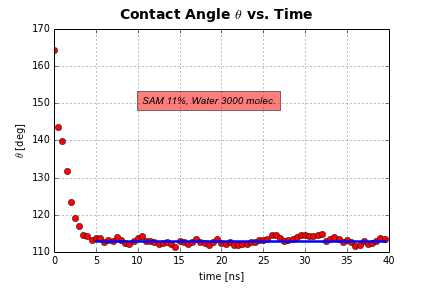
\includegraphics[width=95mm]{thetas11w3000}
}
\subfloat{
  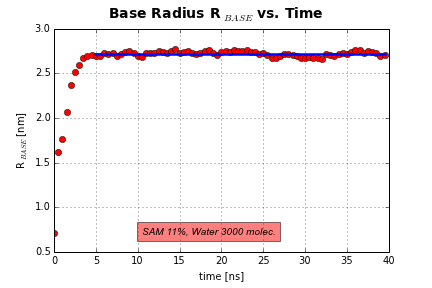
\includegraphics[width=95mm]{rads11w3000}
}
\newline
\subfloat{
  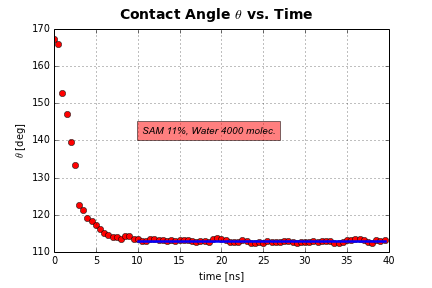
\includegraphics[width=95mm]{thetas11w4000}
}
\subfloat{
  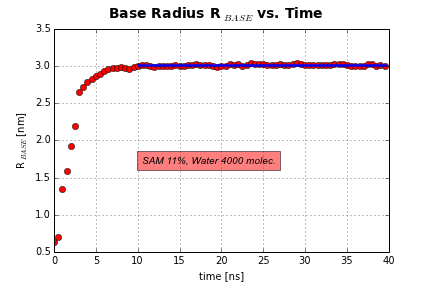
\includegraphics[width=95mm]{rads11w4000}
}
\newline
\subfloat{
  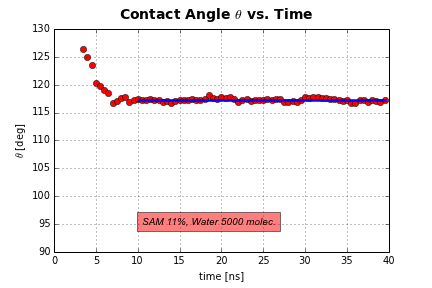
\includegraphics[width=95mm]{thetas11w5000}
}
\subfloat{
  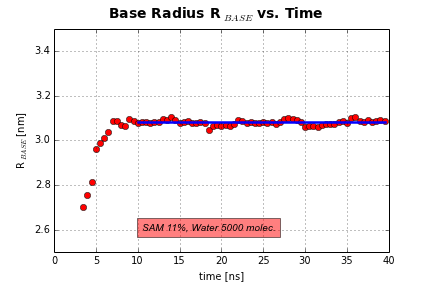
\includegraphics[width=95mm]{rads11w5000}
}
\end{figure}
\begin{figure}
\subfloat{
  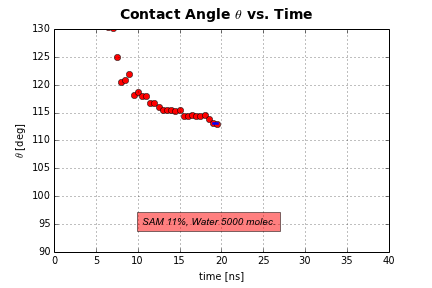
\includegraphics[width=95mm]{thetas11w6500}
}
\subfloat{
  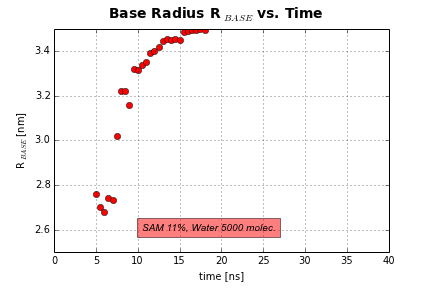
\includegraphics[width=95mm]{rads11w6500}
}
\newline
\subfloat{
  \includegraphics[width=95mm]{thetas11w7000}
}
\subfloat{
  \includegraphics[width=95mm]{rads11w7000}
}
\newline
\subfloat{
  \includegraphics[width=95mm]{thetas11w8000}
}
\subfloat{
  \includegraphics[width=95mm]{rads11w8000}
}
\newline
\subfloat{
  \includegraphics[width=95mm]{thetas11w9000}
}
\subfloat{
  \includegraphics[width=95mm]{rads11w9000}
}
\end{figure}
\begin{figure}
\subfloat{
  \includegraphics[width=95mm]{thetas11w10000}
}
\subfloat{
  \includegraphics[width=95mm]{rads11w10000}
}
%\centering
\newline
{\Large SAMs with 17\% OH-coverage.}
\newline
\subfloat{
  \includegraphics[width=95mm]{thetas17w1000}
}
\subfloat{
  \includegraphics[width=95mm]{rads17w1000}
}
\newline
\subfloat{
  \includegraphics[width=95mm]{thetas17w2000}
}
\subfloat{
  \includegraphics[width=95mm]{rads17w2000}
}
\newline
\subfloat{
  \includegraphics[width=95mm]{thetas17w3000}
}
\subfloat{
  \includegraphics[width=95mm]{rads17w3000}
}
\end{figure}
\begin{figure}
\subfloat{
  \includegraphics[width=95mm]{thetas17w4000}
}
\subfloat{
  \includegraphics[width=95mm]{rads17w4000}
}
\newline
\subfloat{
  \includegraphics[width=95mm]{thetas17w5000}
}
\subfloat{
  \includegraphics[width=95mm]{rads17w5000}
}
\newline
\subfloat{
  \includegraphics[width=95mm]{thetas17w6500}
}
\subfloat{
  \includegraphics[width=95mm]{rads17w6500}
}
\newline
\subfloat{
  \includegraphics[width=95mm]{thetas17w7000}
}
\subfloat{
  \includegraphics[width=95mm]{rads17w7000}
}
\end{figure}
\begin{figure}
\subfloat{
  \includegraphics[width=95mm]{thetas17w8000}
}
\subfloat{
  \includegraphics[width=95mm]{rads17w8000}
}
\newline
\subfloat{
  \includegraphics[width=95mm]{thetas17w9000}
}
\subfloat{
  \includegraphics[width=95mm]{rads17w9000}
}
\newline
\subfloat{
  \includegraphics[width=95mm]{thetas17w10000}
}
\subfloat{
  \includegraphics[width=95mm]{rads17w10000}
}
\end{figure}

\begin{figure}
{\Large Macroscopic Contact Angle}
{\Large $\Theta_{mac}$} 
{\Large and Line Tension}
{\Large $\sigma$}
{\Large from \newline $\cos( \Theta_{mic})  = \cos ( \Theta_{mac}) - \frac{ \sigma}{ \gamma_{LV}} \frac{1}{R_{BASE}}$, \newline where $\gamma_{LV} =52.7 mN/m$}
{\Large and}
{\Large $ \Theta_{mic}$}
{\Large is the Microscopic Contact Angle. }
\newline
\subfloat{
  \includegraphics[width=95mm]{theta_r_s0.png}
}
\subfloat{
  \includegraphics[width=95mm]{theta_r_s5.png}
}
\newline
\subfloat{
  \includegraphics[width=95mm]{theta_r_s11.png}
}
\subfloat{
  \includegraphics[width=95mm]{theta_r_s17.png}
}
\newline
\newline
{\Large Contact Angle and Line Tension vs OH-Percentage}
\newline
\subfloat{
  \includegraphics[width=95mm]{C_Angles_OH.png}
}
\subfloat{
  \includegraphics[width=95mm]{Sigma_OH.png}
}
\end{figure}

\end{document}

